%%%%%%%%%%%%%%%%%%%%%%%%%%%%%%%%%%%%%%%% Blabla %%%%%%%%%%%%%%%%%%%%%%%%%%%%%%%%%%%%%%%%%%%%%%%%%%%%%%
\documentclass[lang=english]{tumposting}

%\setcounter{tocdepth}{3}
\setcounter{secnumdepth}{0}

\usepackage[utf8]{inputenc}
\usepackage[T1]{fontenc}

\usepackage{helvet}
\renewcommand*\familydefault{\sfdefault}

\usepackage{setspace}
%\setstretch{1.5}

\usepackage{amsmath}

\usepackage{pdfpages}

\usepackage{url}

\usepackage{tikz,graphicx,wrapfig}
\graphicspath{{./Images/}}

\usepackage{caption}
\captionsetup[figure]{labelformat=empty}

\usepackage{subfigure}

\usepackage{longtable}

\usepackage{caption}
\renewcommand{\captionfont}{\footnotesize}

\usepackage[square,comma,sort&compress]{natbib}

\usepackage[breaklinks=true,bookmarks=false]{hyperref}
\usepackage{cleveref}

\usepackage[title]{appendix}

\usepackage{blindtext}



%%%%%%%%%%%%%%%%%%%%%%%%%%%%%%%%%%%%%%%%%%%%%%%%%%%%%%%% Title %%%%%%%%%%%%%%%%%%%%%%%%%%%%%%%%%%%%%%%%%%%%%%%%%%%%%%%%%%%%%%%%

\subject{\raggedright {\huge{{\color{tumgray}{Job Posting: Student Research Assistant}}}}}
\title{\raggedright {\Huge{{\color{tumblue}{Generating Datasets from Video Games}}}}}
\date{}


\begin{document}	
\pagestyle{empty}

\maketitle
	
	
	
%%%%%%%%%%%%%%%%%%%%%%%%%%%%%%%%%%%%%%%%%%%%%%%%%%%%%%%% Document %%%%%%%%%%%%%%%%%%%%%%%%%%%%%%%%%%%%%%%%%%%%%%%%%%%%%%%%%%%%%%%%

\vspace*{-20mm}
\subsection{Description}
\begin{wrapfigure}{r}{0mm}
	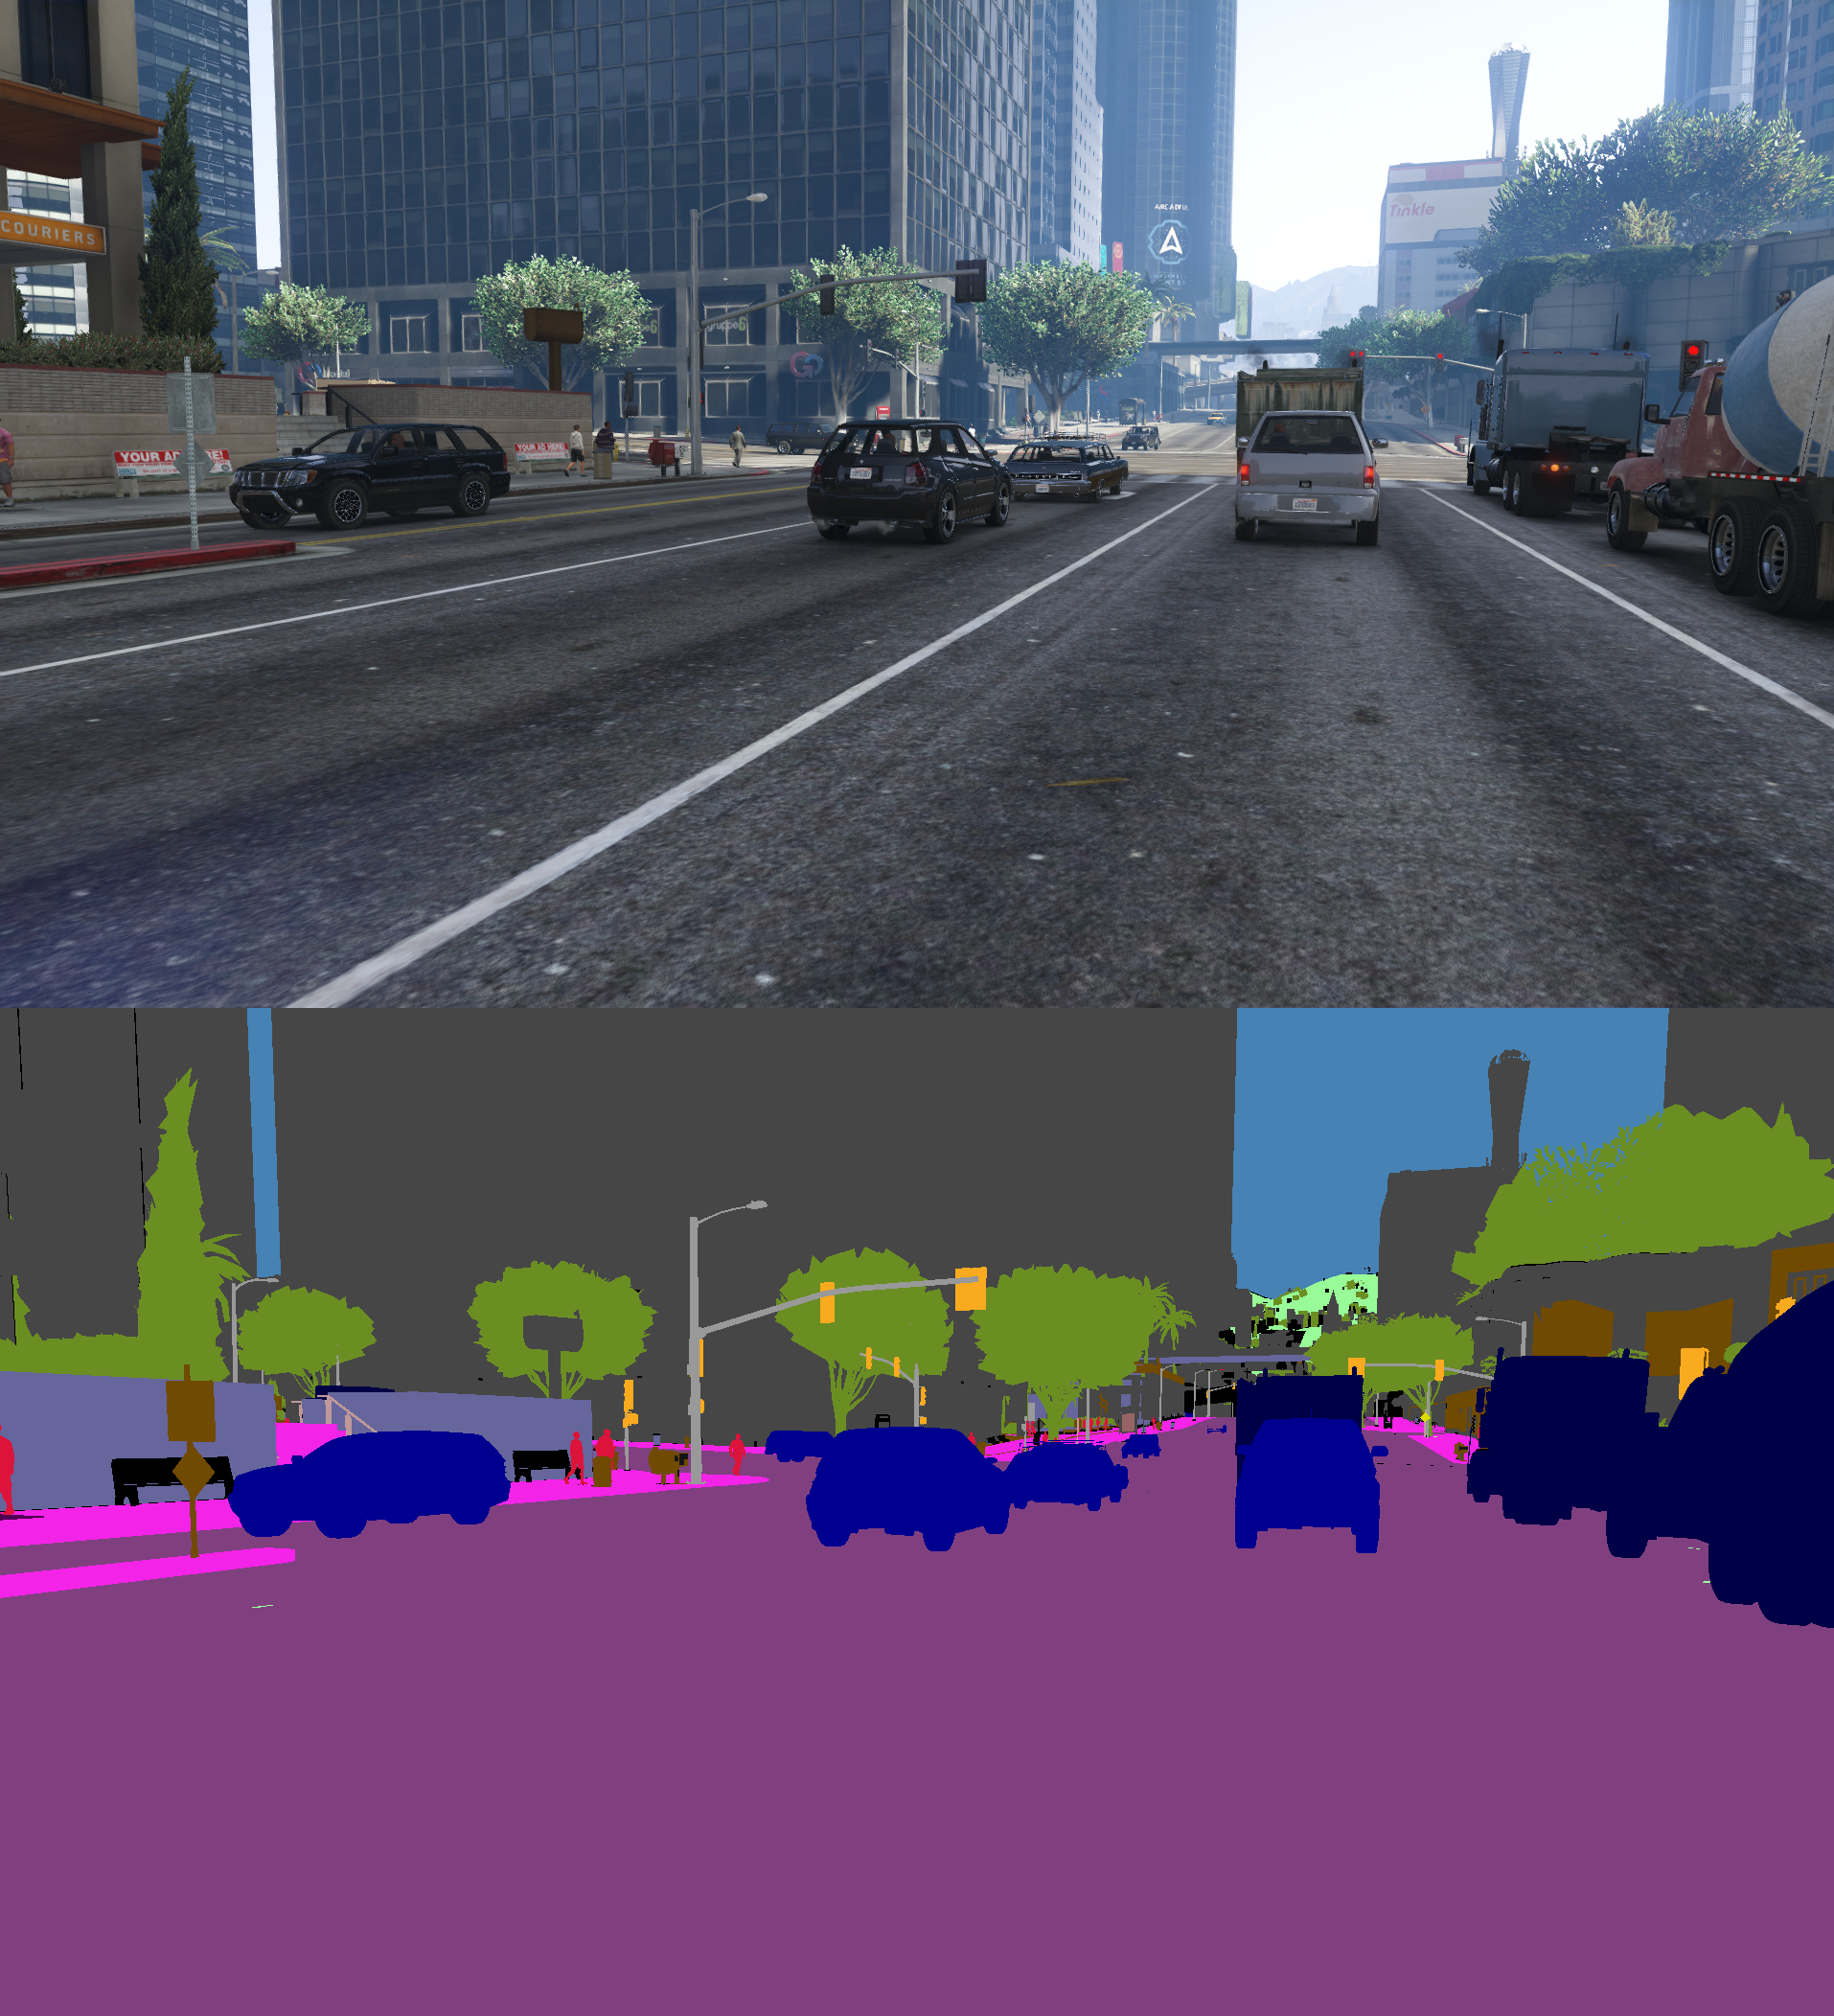
\includegraphics[width=0.45\textwidth]{PlayingForData}
	\caption[]{{\tiny{Image: example image from Playing for Data dataset [Richter et al., 2016]}}}
\end{wrapfigure}
State of the art machine learning models for object detection and classification tasks require a large amount of labeled data, especially when trained in a supervised manner. 
For these models not only the size of the dataset is of great importance, but also the variety and structure of the data. 
Recent developments have shown, that synthetically generated data can be part of the solution to this problem.
Since many of today's 3d video games provide photo-realistic environments, several new approaches came up, making use of such video games to gather additional data. \\

\noindent
In our research, we are learning a model to predict future video frames based on a given input sequence.
The main application of our model will be to predict traffic scenes including the behavior of traffic participants.
Under these constraints, we want to combine existing publicly available datasets of real world traffic scenes with similar synthetic data. \\

\noindent
The focus of your work as a student research assistant will be to make use of existing approaches to collect a new dataset of labeled video sequences from video games.
The most relevant approaches for our research extract data from the popular game Grand Theft Auto V (GTA V).
It is therefore recommended to use GTA V in your work, however, the project is not limited to this particular game. 
For the purpose of generating data it is highly appreciated, if you have a basic understanding of the rendering process in video games. 
Also, good programming skills in Python are essential. 
All further details will be settled in person.


\subsection{Requirements}
\begin{itemize}
	\item Interest in video games and basic idea of the rendering process in 3D video games
	\item Advanced programming skills (Python)
	\item Ability to work independently
\end{itemize}

\vspace*{2mm}
\hrulefill

\subsection{Contact}

\begin{tabular}[c]{ll}
	Dr. rer. nat. Marco Körner	& Chair of Remote Sensing Technology\\
	M. Sc. Sandra Aigner		& Arcisstr. 21 \\
	M. Sc. Lukas Liebel			& 80333, München\\
								& \\
	\{lukas.liebel, sandra.aigner, marco.körner\}@tum.de &
\end{tabular}


\end{document}
